\documentclass[a4paper, 10pt, final]{article}
\usepackage{sip_report}

%% \def\mytitle{Signal and Image Processing 2010}
%% \def\mysubtitle{Handin of mandatory excercise 1}
%% \def\myauthor{Ulrik Bonde}
%% \def\mymail{\mailto{bonde@diku.dk}}
%% \def\mydate{\today}

\title{Signal and Image Processing 2010 \\ Mandatory hand-in exercise 3}
\author{Michael Andersen}
\date{\today}

%% \title{\mytitle}
%% \subtitle{\mysubtitle}

%% \author{\myauthor{} - \mymail}
%% \date{\mydate}

\hypersetup{
colorlinks,%
citecolor=black,%
filecolor=black,%
linkcolor=black,%
urlcolor=black,%
bookmarksopen=false,
pdftitle={Signal and Image Processing 2010 - Mandatory exercise 3},
pdfauthor={Michael Andersen}
}

\begin{document}
\maketitle

\subsection*{Question 3.1}

We are to implement ideal low- and highpass filter, the butterworth
filter and (optionally) the high-frequency-emphasis filter. Then we
are to apply the filters to the image \emph{unix.tiff} and
(optionally) to simply visual inspection to \emph{square.tiff}.

All the filters work in the frequency domain, therefore they need to
be applied to an already fourier transformed image. After applying the
filter in the frequency domain, we need to inverse fourier transform
the image to see the result.

The filters work by using a \textit{cut-off} distance from the center
of the fourier transformed image, because the center of the fourier
transformed image contains low frequencies and higher frequencies the
farther away from the center one gets. The \textit{cut-off} distance
regulates what frequencies that are allowed to pass through the
filter. Using a lowpass filter only low frequencies are allowed to
pass through.

The ideal lowpass filter is defined as follows:

\begin{equation*}
    h(u, v) = \left\{ \begin{array}{l l l}
        1 & \mbox{if} & D(u, v) < D_0\\
        0 & \mbox{otherwise} &
    \end{array}\right.
\end{equation*}

Where $D(u, v) = \sqrt{(u - i)^{2} + (v - j)^{2}}$, having $i =
\nicefrac{M}{2}$ and $j = \nicefrac{N}{2}$. The values $i$ and $j$
defines the center of the image.

\begin{figure}[!htbp]
  \centering
  \subfloat[]{
\includegraphics[width=0.30\textwidth]{./images/square}} \
  \subfloat[]{
\includegraphics[width=0.30\textwidth]{./images/square_ideal_low_filter_30}} \\
  \subfloat[]{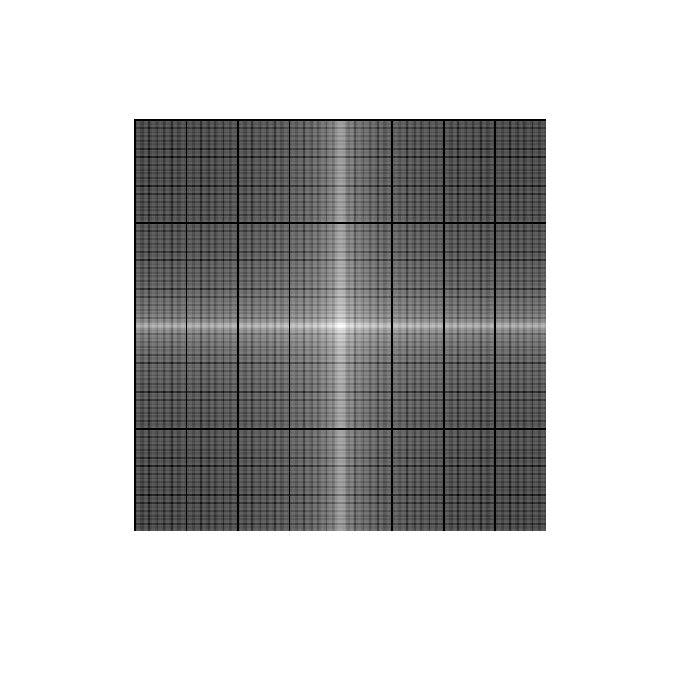
\includegraphics[width=0.4\textwidth]{./images/square_ft}} \
  \subfloat[]{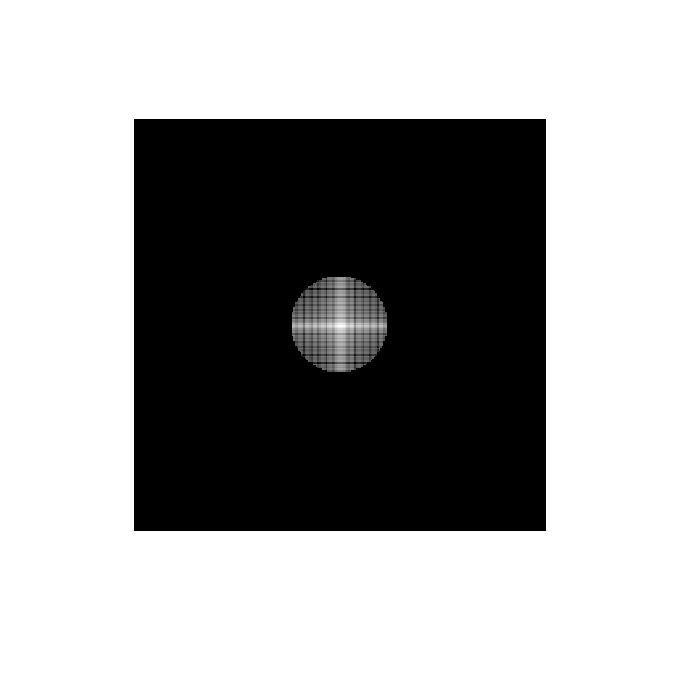
\includegraphics[width=0.4\textwidth]{./images/square_ftmod_low}} \\
  \subfloat[]{
\includegraphics[width=0.4\textwidth]{./images/square_ideal_low_result_30}}
  \caption{a) Image 1, b) Fourier transform of image 1, c) Image 2, d) Fourier transform of image 2}
  \label{fig:lowpass30}
\end{figure}

Figure \ref{fig:lowpass30} shows a ideal lowpass filter with
\textit{cut-off} set to $30$, it is easy to the the ripple effect
caused by ideal lowpass filter.

\begin{figure}[!htbp]
  \centering
  \subfloat[]{
\includegraphics[width=0.4\textwidth]{./images/square_ideal_high_filter_30}} \
  \subfloat[]{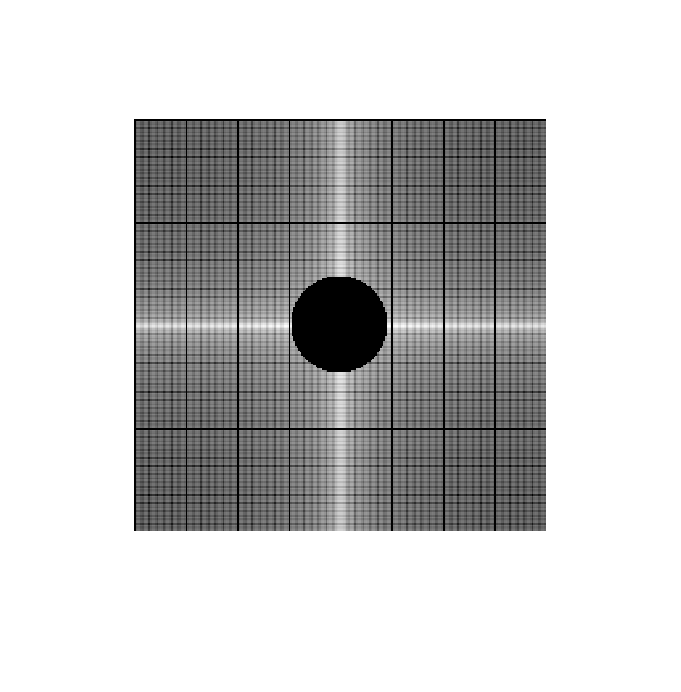
\includegraphics[width=0.4\textwidth]{./images/square_ftmod_high}} \\
  \subfloat[]{
\includegraphics[width=0.4\textwidth]{./images/square_ideal_high_result_30}}
  \caption{a) Image 1, b) Fourier transform of image 1, c) Image 2, d) Fourier transform of image 2}
  \label{fig:highpass30}
\end{figure}

Figure \ref{fig:highpass30} show a ideal highpass filter with
\textit{cut-off} set to $30$ as the lowpass. Again it is easy to the
ripple effect, when using a highpass filter it is worth mentioning
that most of the structure in the image disappears. This is what
causes the white parts to become black. This ripple effect is caused
by the \emph{sinc} function.

\begin{figure}
  \centering 
\includegraphics[width=0.7\textwidth]{./images/unix}
  \label{fig:unix_original}
\end{figure}

\begin{figure}[!htbp]
  \centering
  \subfloat[Cut-off $= 5$]{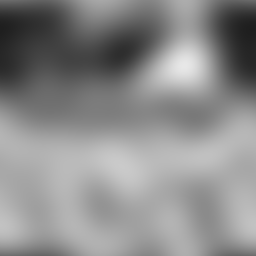
\includegraphics[width=0.30\textwidth]{./images/unix_ideal_low_result_5}} \
  \subfloat[Cut-off $= 20$]{
\includegraphics[width=0.30\textwidth]{./images/unix_ideal_low_result_20}} \
  \subfloat[Cut-off $= 50$]{
\includegraphics[width=0.30\textwidth]{./images/unix_ideal_low_result_50}}
  \caption{Ideal lowpass filter for varies cut-off values}
  \label{fig:unix_lowpass}
\end{figure}



\begin{figure}[!htbp]
  \centering
  \subfloat[Cut-off $= 5$]{
\includegraphics[width=0.30\textwidth]{./images/unix_ideal_high_result_5}} \
  \subfloat[Cut-off $= 20$]{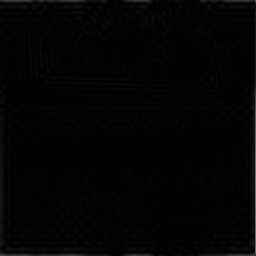
\includegraphics[width=0.30\textwidth]{./images/unix_ideal_high_result_20}} \
  \subfloat[Cut-off $= 50$]{
\includegraphics[width=0.30\textwidth]{./images/unix_ideal_high_result_50}}
  \caption{Ideal highpass filter for varies cut-off values.}
  \label{fig:unix_high}
\end{figure}

\begin{figure}
  \centering
  
\includegraphics[width=0.60\textwidth]{./images/unix_ideal_high_result_2}
  \caption{Ideal highpass filter, using cut-off $= 2$.}
  \label{fig:unix_high2}
\end{figure}

We are now done with the ideal filters, and move on to the butterworth
filter. Butterworth filter is smoother than ideal filters as it does
not have the sudden edge in the filter but have a smoother transition.

The butterworth filter is defined as:
\begin{equation*}
    h(u, v) = \frac{1}{1 + \left[ \frac{D(u,v)}{D_{0}}\right]^{2n}} 
\end{equation*}

Again we consider the original image from figure
\ref{fig:unix_original}

\begin{figure}[!htbp]
  \centering
  \subfloat[Cut-off $= 5$]{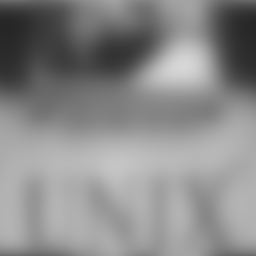
\includegraphics[width=0.30\textwidth]{./images/unix_butter_low_result_5}} \
  \subfloat[Cut-off $= 20$]{
\includegraphics[width=0.30\textwidth]{./images/unix_butter_low_result_20}} \
  \subfloat[Cut-off $= 50$]{
\includegraphics[width=0.30\textwidth]{./images/unix_butter_low_result_50}}
  \caption{Butterworth filter for varies cut-off values}
  \label{fig:unix_butterworth}
\end{figure}



% Shows how listing is done, Bonde style!!!
\begin{lstlisting}[caption={Calculating and showing the Fourier
    transform of an image using MATLAB.}, captionpos=b,
    label={lst:fft_matlab}, float=b, numbers=none]
% Read the original image
I = imread('../../../../square.tiff');

% Perform Fourier transform and shift the image
ft = fft2(I);
ft = fftshift(ft);

% Show the original image
imshow(I);

% Show the Fourier transformed image
% We use the absolute value because of complex numbers
% We use log to scale large values
figure, imshow(log(abs(1 + ft)), []);
\end{lstlisting}


%% \begin{figure}[!htbp]
%%   \centering
%%   \subfloat[]{\includegraphics[width=0.4\textwidth]{./images/}}
%%   \subfloat[]{\includegraphics[width=0.4\textwidth]{./images/}} \\
%%   \subfloat[]{\includegraphics[width=0.4\textwidth]{./images/}}
%%   \subfloat[]{\includegraphics[width=0.4\textwidth]{./images/}}
%%   \caption{a) Image 1, b) Fourier transform of image 1, c) Image 2, d) Fourier transform of image 2}
%%   \label{fig:exercise2_1a}
%% \end{figure}


%% \begin{figure}[!htbp]
%% \centering
%% \subfloat[]{\includegraphics[width=0.4\textwidth]{./images/}}
%% \subfloat[]{\includegraphics[width=0.4\textwidth]{./images/}}
%% \caption{a) Fourier transform with padding of image 1 in figure \ref{fig:exercise2_1a}, b) Fourier transform with padding of image 2 in figure \ref{fig:exercise2_1a} }
%% \label{fig:exercise2_1b}
%% \end{figure}

\newpage

\subsection*{Question 3.2}

We let $I(x,y)$ be an image of size $M \times M$ and $f(x,y)$ be a
seperable filter of size $N \times N$. We are to calculate how many
multiplications it requires to calculate $I \star f$ in the spatial
domain.

I start by considering the \emph{naive} situation, where $f$ is not
seperable. As we need to multiply every pixel within $I$ with every
pixel within the filter, this would require $M^{2}N^{2}$
multiplication. This very fast becomes infeasiable for large values of
$M$ and $N$.

Under the assumption that $f$ is seperable we can seperate the filter
and convolve the rows and columns of $I$ seperately. As $I$ have $M$
rows with $M$ pixels each and $M$ columns with $M$ pixels each. Using
that the filter is seperable it because $1$-D (i.e. linear in its
size), we have $N$ multiplications for rows and $N$ multiplications
for columns in the spatial domain this results in ($I
\star_{\textrm{s} f}$ denotes convolution within the spatial domain)

\begin{align*}
  I \star_{\textrm{s}} f & = 2(M(MN)) \\
  & = 2M^{2}N
\end{align*}

We now need to answer the same question in the frequency domain.

Now considering the fourier domain and the assumption that the
transform of a signal of length $L$ takes $L \log{(L)}$
multiplications. The filter is still assumed seperable, therefore we
make the same arguments as before. As the image has $M$ rows with $M$
pixel each and $M$ columns with $M$ pixels each we need $2(M^{2}
\log{(M)})$ to transform the image. We need to pad the filter to make
it the same size as the image (to perform the pointwise complex
multiplication in the fourier domain) and also fourier transform it
this is another $2(M^{2} \log{(M)})$. When transformed the convolution
is just a pointwise multiplication of $\mathcal{F}(I)$ and
$\mathcal{F}(f)$ this requires $M^{2}$ multiplications. Under the
assumption that the inverse fourier transformed can be performed with
the same number of multiplications as the fourier transform, we need
another $2(M^{2} \log{(M)})$ to inverse fourier transform the
image. We do not need the filter anymore, so this can be disregarded
when performing the inverse fourier transform. Therefore within the
frequency domain the result is ($I \star_{\textrm{f} f}$ denotes
convolution within the frequency domain)

\begin{align*}
  I \star_{\textrm{f}} f & = 2(2(M^{2}\log{(M)})) + M^{2} + 2(M^{2}\log{(M)})) \\
  & = 6M^{2}\log{(M)} + M^{2}
\end{align*}

We are now to answer then it is advantageous to perform the
convolution in the spatial domain versus in the frequency domain.

In order to solve this we need to solve the inequality $(I
\star_{\textrm{f}} f) < (I \star_{\textrm{s}} f)$ with respect to the
filter size $N$.

\begin{align}
  \label{eq:1}6M^{2}\log{(M)} + M^{2} & < 2M^{2}N \\
  \label{eq:2} 3 \log{(M)} + \frac{1}{2} & < N
\end{align}

This is done by dividing inequality \ref{eq:1} through with $2M^{2}$,
resulting in inequality \ref{eq:2}.

We are now to consider when we are dealing with an already known
fourier transform.

As we do not need to fourier transform the filter in the first place,
this reduces inequality \ref{eq:1} to \ref{eq:3} resulting in
\ref{eq:4}

\begin{align}
  \label{eq:3}4M^{2}\log{(M)} + M^{2} & < 2M^{2}N \\
  \label{eq:4}2\log{(M)} + \frac{1}{2} & < N
\end{align}

For convolution in the frequency domain we only need to require \ref{eq:4}.

\subsection*{Question 3.3}

We are to try various form of restoration on the images
\emph{noisy.tiff} and \emph{berlinger.tiff}.

%% \begin{figure}[!htbp]
%%   \centering
%%   \subfloat[]{\includegraphics[width=0.5\textwidth]{./images/}}
%%   \subfloat[]{\includegraphics[width=0.5\textwidth]{./images/}}
%%   \caption{Shows the two signals.}
%%     \label{fig:q2_3a}
%% \end{figure}


%%%%%%%%%%%%%%%%%%%%%%%%%%%%%%%%%%%%%%%%%%%%%%%%%%%%%%%%%%%%%%%%%%%%
% Formal stuff

%\bibliographystyle{abbrvnat}
%\bibliography{bibliography}
%\addcontentsline{toc}{chapter}{Litteratur}

\end{document}

% vim: set tw=72 spell spelllang=en:
